\let\negmedspace\undefined
\let\negthickspace\undefined
\documentclass[journal,12pt,onecolumn]{IEEEtran}
\usepackage{cite}
\usepackage{amsmath,amssymb,amsfonts,amsthm}
\usepackage{algorithmic}
\usepackage{graphicx}
\usepackage{textcomp}
\usepackage{xcolor}
\usepackage{txfonts}
\usepackage{listings}
\usepackage{enumitem}
\usepackage{mathtools}
\usepackage{gensymb}
\usepackage[breaklinks=true]{hyperref}
\usepackage{tkz-euclide} % loads  TikZ and tkz-base
\usepackage{listings}



\newtheorem{theorem}{Theorem}[section]
\newtheorem{problem}{Problem}
\newtheorem{proposition}{Proposition}[section]
\newtheorem{lemma}{Lemma}[section]
\newtheorem{corollary}[theorem]{Corollary}
\newtheorem{example}{Example}[section]
\newtheorem{definition}[problem]{Definition}
%\newtheorem{thm}{Theorem}[section] 
%\newtheorem{defn}[thm]{Definition}
%\newtheorem{algorithm}{Algorithm}[section]
%\newtheorem{cor}{Corollary}
\newcommand{\BEQA}{\begin{eqnarray}}
\newcommand{\EEQA}{\end{eqnarray}}
\newcommand{\define}{\stackrel{\triangle}{=}}
\theoremstyle{remark}
\newtheorem{rem}{Remark}
%\bibliographystyle{ieeetr}
\begin{document}
%
\providecommand{\pr}[1]{\ensuremath{\Pr\left(#1\right)}}
\providecommand{\prt}[2]{\ensuremath{p_{#1}^{\left(#2\right)} }}        % own macro for this question
\providecommand{\qfunc}[1]{\ensuremath{Q\left(#1\right)}}
\providecommand{\sbrak}[1]{\ensuremath{{}\left[#1\right]}}
\providecommand{\lsbrak}[1]{\ensuremath{{}\left[#1\right.}}
\providecommand{\rsbrak}[1]{\ensuremath{{}\left.#1\right]}}
\providecommand{\brak}[1]{\ensuremath{\left(#1\right)}}
\providecommand{\lbrak}[1]{\ensuremath{\left(#1\right.}}
\providecommand{\rbrak}[1]{\ensuremath{\left.#1\right)}}
\providecommand{\cbrak}[1]{\ensuremath{\left\{#1\right\}}}
\providecommand{\lcbrak}[1]{\ensuremath{\left\{#1\right.}}
\providecommand{\rcbrak}[1]{\ensuremath{\left.#1\right\}}}
\newcommand{\sgn}{\mathop{\mathrm{sgn}}}
\providecommand{\abs}[1]{\left\vert#1\right\vert}
\providecommand{\res}[1]{\Res\displaylimits_{#1}} 
\providecommand{\norm}[1]{\left\lVert#1\right\rVert}
%\providecommand{\norm}[1]{\lVert#1\rVert}
\providecommand{\mtx}[1]{\mathbf{#1}}
\providecommand{\mean}[1]{E\left[ #1 \right]}
\providecommand{\cond}[2]{#1\middle|#2}
\providecommand{\fourier}{\overset{\mathcal{F}}{ \rightleftharpoons}}
\newenvironment{amatrix}[1]{%
  \left(\begin{array}{@{}*{#1}{c}|c@{}}
}{%
  \end{array}\right)
}
%\providecommand{\hilbert}{\overset{\mathcal{H}}{ \rightleftharpoons}}
%\providecommand{\system}{\overset{\mathcal{H}}{ \longleftrightarrow}}
	%\newcommand{\solution}[2]{\textbf{Solution:}{#1}}
\newcommand{\solution}{\noindent \textbf{Solution: }}
\newcommand{\cosec}{\,\text{cosec}\,}
\providecommand{\dec}[2]{\ensuremath{\overset{#1}{\underset{#2}{\gtrless}}}}
\newcommand{\myvec}[1]{\ensuremath{\begin{pmatrix}#1\end{pmatrix}}}
\newcommand{\mydet}[1]{\ensuremath{\begin{vmatrix}#1\end{vmatrix}}}
\newcommand{\myaugvec}[2]{\ensuremath{\begin{amatrix}{#1}#2\end{amatrix}}}
\providecommand{\rank}{\text{rank}}
\providecommand{\pr}[1]{\ensuremath{\Pr\left(#1\right)}}
\providecommand{\qfunc}[1]{\ensuremath{Q\left(#1\right)}}
	\newcommand*{\permcomb}[4][0mu]{{{}^{#3}\mkern#1#2_{#4}}}
\newcommand*{\perm}[1][-3mu]{\permcomb[#1]{P}}
\newcommand*{\comb}[1][-1mu]{\permcomb[#1]{C}}
\providecommand{\qfunc}[1]{\ensuremath{Q\left(#1\right)}}
\providecommand{\gauss}[2]{\mathcal{N}\ensuremath{\left(#1,#2\right)}}
\providecommand{\diff}[2]{\ensuremath{\frac{d{#1}}{d{#2}}}}
\providecommand{\myceil}[1]{\left \lceil #1 \right \rceil }
\newcommand\figref{Fig.~\ref}
\newcommand\tabref{Table~\ref}
\newcommand{\sinc}{\,\text{sinc}\,}
\newcommand{\rect}{\,\text{rect}\,}
%%
%	%\newcommand{\solution}[2]{\textbf{Solution:}{#1}}
%\newcommand{\solution}{\noindent \textbf{Solution: }}
%\newcommand{\cosec}{\,\text{cosec}\,}
%\numberwithin{equation}{section}
%\numberwithin{equation}{subsection}
%\numberwithin{problem}{section}
%\numberwithin{definition}{section}
%\makeatletter
%\@addtoreset{figure}{problem}
%\makeatother

%\let\StandardTheFigure\thefigure
\let\vec\mathbf

\bibliographystyle{IEEEtran}





\bigskip

\renewcommand{\thefigure}{\theenumi}
\renewcommand{\thetable}{\theenumi}
%\renewcommand{\theequation}{\theenumi}

Q:Two APs have the same common difference.The difference between their $100${th} terms is 100,what is the difference between their $1000${th} terms?

\solution

\begin{align}
x(n) &= \{x(0)+nd\}u(n) \\
 x(99) - y(99) &= 100 \\
\implies (x(0) + 99d) - (y(0) + 99d) &= 100
 \\
\implies x(0) - y(0) &= 100
\end{align}

\begin{align}
x(n) - y(n) &= (x(0) + nd) - (y(0) + nd)\\
&= x(0) - y(0) \\
&= 100  
\end{align}
Therefore,the difference between the 1000th terms of two given APs is 100.\\

We know that,

The Z-transform of a discrete signal $x(n)$ is given by:
\[ X(z) = \mathcal{Z}\{x(n)\} = \sum_{n=-\infty}^{\infty} x(n)z^{-n} \]
\\ Considering x(n-1) and y(n-1) as $n^{th}$ terms of the APs(Arithmetic Progressions), Z-transform for x(n) and y(n) can be given by
\begin{align}
X(z) = \mathcal{Z}\{x(n)\} 
&=\sum_{n=-\infty}^{\infty} x(n)z^{-n} \\
&=\sum_{n=0}^{\infty}x(n)z^{-n} \\
&=x(0)U(z) + d[-z \frac {d(U(z))}{dz}] \\
&=\frac{x(0)}{1-z^{-1}} + \frac{dz^{-1}}{(1-z^{-1})^2} \hspace{5pt} ROC: |z|>1\\
X(z)&= \frac{x(0)}{1-z^{-1}} + \frac{dz^{-1}}{(1-z^{-1})^2} \hspace{5pt} ROC: |z|>1\\
Y(z)&= \frac{y(0)}{1-z^{-1}} + \frac{dz^{-1}}{(1-z^{-1})^2} \hspace{5pt} ROC: |z|>1
\end{align}
\begin{table}[!ht]
    \centering
        
      \begin{tabular}{|c|c|c|} 
      \hline
\textbf{Variable}& \textbf{Description}& \textbf{Value}\\\hline
         $x(n)$& $n^{th}$ term of X&none\\\hline
          $y(n)$& $n^{th}$ term of Y&none\\\hline
          $d$&common difference between the terms of AP&none\\\hline
          $x(n)-y(n)$& difference of $n^{th}$ terms of X and Y &$x(99)-y(99)=100$ \\ \hline
         
    \end{tabular}


    \caption{input parameters}
    \label{tab:10_5_3_12}
\end{table}

\begin{align}
x(n)&= \{101,106,111,...\} \\
y(n)&= \{1,6,11,... \} 
\end{align}


\begin{figure}
    \centering
    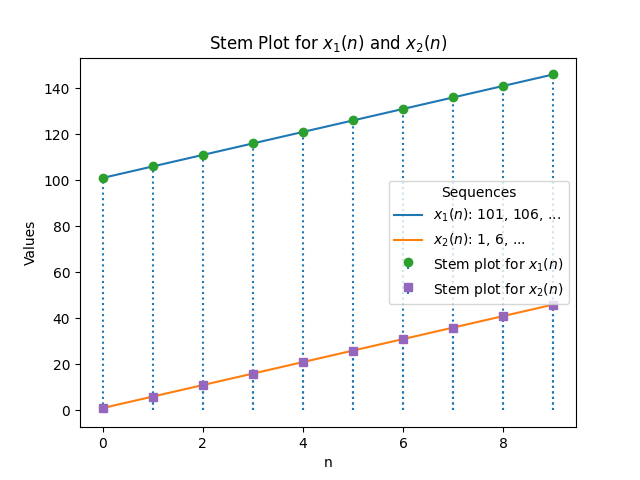
\includegraphics{./figs/fig2.png}
    \caption{ }
    \label{fig:x(n) & y(n) }
\end{figure}

\begin{figure}
    \centering
    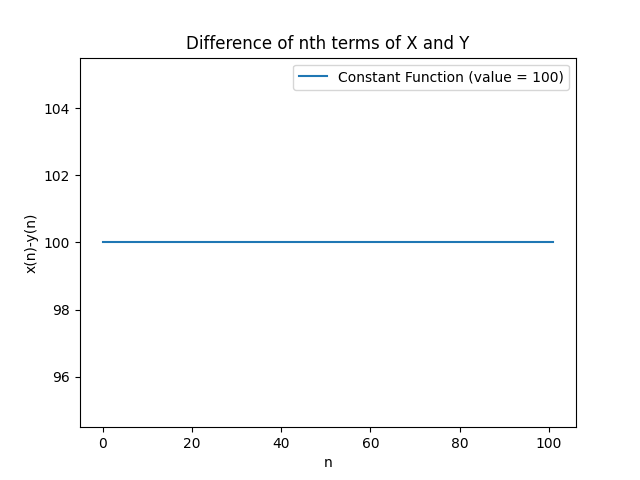
\includegraphics{./figs/fig1.png}
    \caption{ }
    \label{fig:difference of x(n) & y(n) }
\end{figure}
\end{document}
